\section{Introduction}
\label{sec:introduction}
\textbf{[To review]}
The CLEF~2026 CheckThat!~Lab Task~1 frames scientific claim retrieval as
a low-resource, cross-lingual ad-hoc retrieval problem.
As shown in Figure~\ref{fig:task-definition}, given a tweet — written mainly in English, German,
or French — that implicitly cites a scientific paper, the system must rank a fixed corpus
of 10{,}000~scientific papers so that the cited paper appears as high as possible in the
returned list.
The task is hard for two reasons: (i)~tweets are short, noisy, and
multilingual, while abstracts are long, technical, and predominantly
written in English; and (ii)~a German or French query may
correspond to an English target paper, so monolingual retrieval breaks
the assumption that query and document share a vocabulary.

We approach this problem as an opportunity to systematically apply and
evaluate core IR techniques — from sparse lexical models to dense
neural retrieval — against a real-world, competitive benchmark.
Our experiments investigate the trade-offs between retrieval
effectiveness and computational efficiency under the constraints imposed
by the competition setting.

\begin{figure}
  \centering
  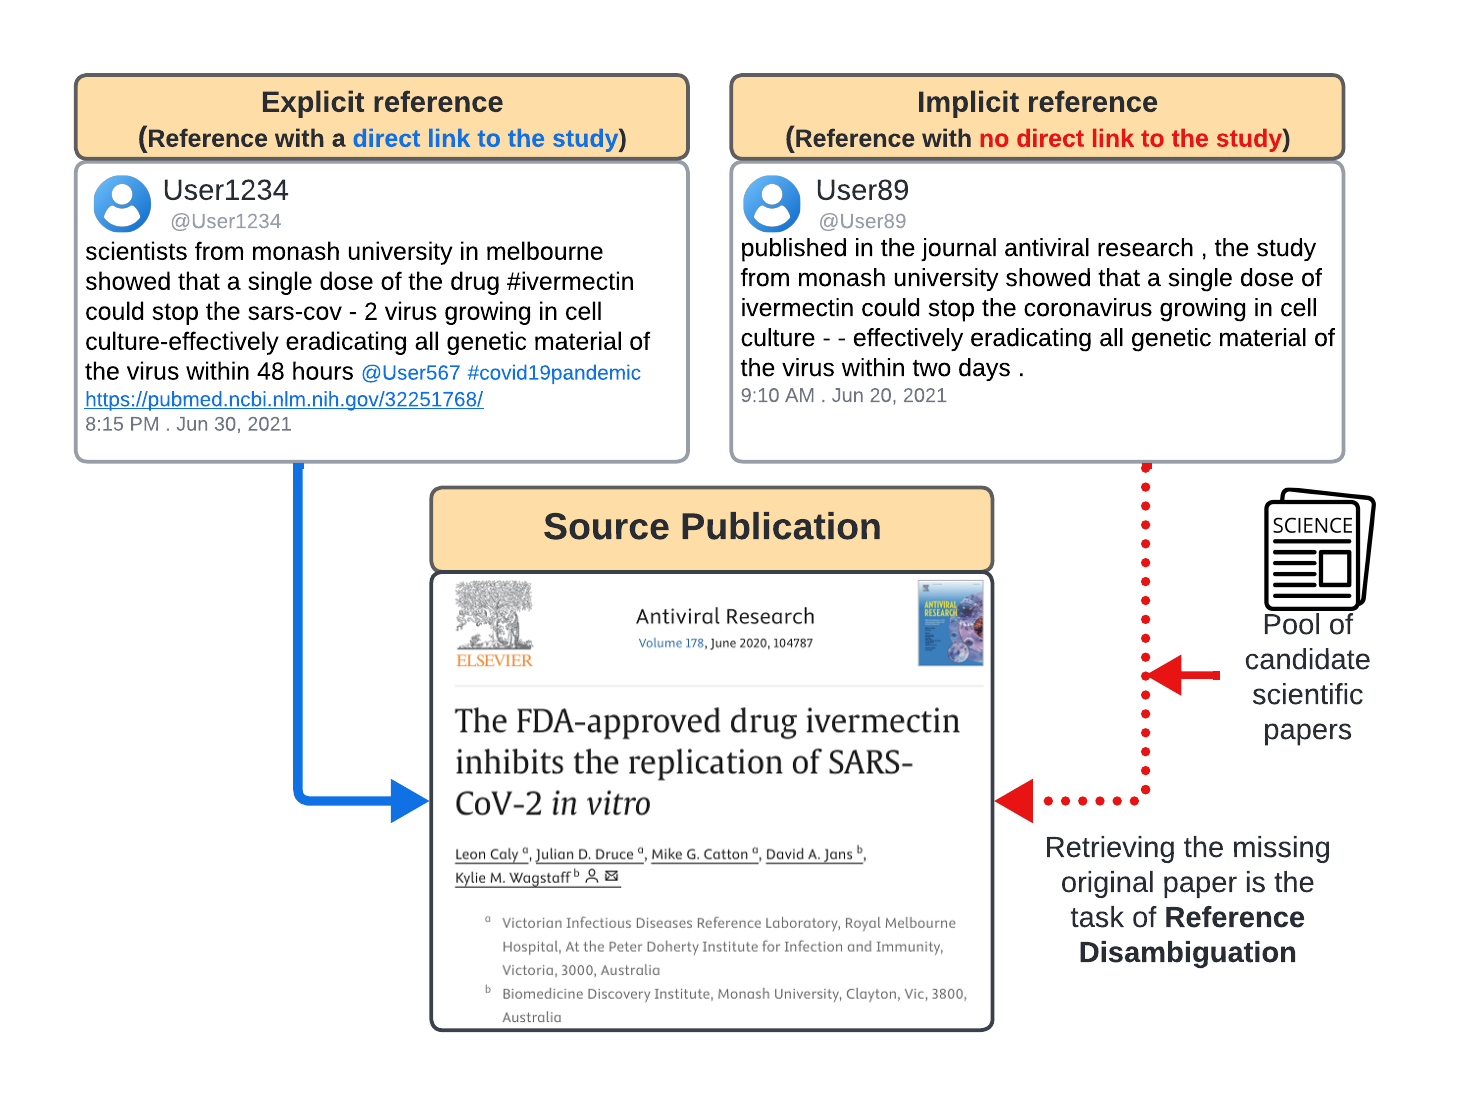
\includegraphics[width=0.6\linewidth]{figure/01-figure_example-task.png}
  \caption{An example of the source retrieval task for scientific web claims~\cite{hafid2025disambiguation}.
           Two tweets which the first one (left) has an explicit reference, while the second one implicitly references a scientific paper (right), the system must
           retrieve the cited publication (bottom) from a fixed corpus, adapted from \cite{}}
  \label{fig:task-definition}
\end{figure}

The paper is organized as follows: Section~\ref{sec:methodology} describes our approach;
Section~\ref{sec:setup} explains our experimental setup;
Section~\ref{sec:results} discusses our main findings;
finally, Section~\ref{sec:conclusion} draws conclusions and outlines future work.
\textbf{[To review]}
% TODO: add to bibliography.bib:
%   key: hafid2025disambiguation
%   S. Hafid, Y. S. Kartal, S. Schellhammer, V. Jacot, S. Bringay, S. Dietze, K. Todorov,
%   "Disambiguation of implicit scientific references on X",
%   Proceedings of the 36th ACM Conference on Hypertext and Social Media (2025).
%
%   key: checkthat2026
%   CLEF 2026 CheckThat! Lab Task 1 overview paper (add when published).